% Copyright (c) 2021 ArSysOp and others
%
% This program and the accompanying materials are made available under the
% terms of the Eclipse Public License 2.0 which is available at
% https://www.eclipse.org/legal/epl-2.0/.
%
% SPDX-License-Identifier: EPL-2.0
%
% Contributors:
%     Nikifor Fedorov (ArSysOp)

\documentclass[12pt]{report}

\usepackage{color}
\usepackage[usenames,dvipsnames,svgnames,table]{xcolor}

\usepackage{graphicx}
\graphicspath{{../../i/o/},{../../i/common/}}

\usepackage{hyperref}
\hypersetup{colorlinks=true,
linkcolor=black,
urlcolor=gray}

\usepackage{fancyhdr}
\pagestyle{fancy}
\fancyhf{}
\lhead{
\includegraphics[width=13pt]{glyph}}
\rhead{\leftmark}
\lfoot{\thepage}
\rfoot{Eclipse Passage}
\renewcommand{\chaptermark}[1]{\markboth{#1}{}}
\renewcommand{\headrulewidth}{0.5pt}
\renewcommand{\footrulewidth}{0.5pt}

\fancypagestyle{plain}{
    \fancyhf{}
    \lhead{
\includegraphics[width=13pt]{glyph}}
    \rhead{\leftmark}
    \lfoot{\thepage}
    \rfoot{Eclipse Passage}
    \renewcommand{\headrulewidth}{0.5pt}
    \renewcommand{\footrulewidth}{0.5pt}
}

\setlength{\headheight}{16pt}

\title{Eclipse Passage Operator User Guide}
\author{ArSysOp}
\date{26 June 2021}

\begin{document}

\begin{titlepage}
    \begin{center}
        \vspace*{1cm}

        \Huge \textbf{Eclipse Passage Operator}
        
        \Huge  \textbf{User Guide}

        \vspace{0.5cm}

        \Large  \today

        \vfill

        
\includegraphics[width=5cm]{passage}

        \vfill

        \Large
        ArSysOp
    \end{center}
\end{titlepage}

\tableofcontents
\markboth{Table of Contents}{}

\addcontentsline{toc}{chapter}{Introduction}
\chapter*{Introduction}
\markboth{Introduction}{}

\addcontentsline{toc}{section}{Overview}
\section*{Overview}

\textbf{Eclipse Passage} is a set of tools and libraries providing rich and easily adaptable capabilities to declare and control licensing constraints.
Being an open-source project under Eclipse Foundation, it is entirely developed with Java 11 by the \textit{ArSysOp} company.

This user guide contains a glossary, which gives you base understanding of terms used in Eclipse Passage and two sets of instructions: for developer, who
wants to license some features or entire application with Passage, and for operator, who wants to manage licenses and metadata with the Eclipse Passage Operator.

Happy Reading!

\addcontentsline{toc}{section}{Contribution}
\section*{Contribution}

If you found a mistake in the text or just want to improve this user guide, feel free to contribute on \href{https://github.com/eclipse-passage/passage-docs}{Github} repository.

Also we want to remind that Eclipse Passage is an open-source project, so you can always contribute to the project \href{https://github.com/eclipse-passage/passage}{itself}.

\addcontentsline{toc}{section}{License}
\section*{License}

These materials are made available under the terms of the \href{https://www.eclipse.org/legal/epl-2.0/}{Eclipse Public License 2.0}.

\addcontentsline{toc}{chapter}{Components}
\chapter*{Components}
\markboth{Components}{}

Eclipse Passage consists of three parts:

\addcontentsline{toc}{section}{Licensing Components}
\section*{Licensing Components}

Licensing Components is a set of tools you have to include in your application to be able to declare any licensing logic (For example, what to do if a correct license was not acquired by the licensing framework).
It allows you to restrict unauthorized using of a single feature, bundle or even the whole application.

\addcontentsline{toc}{section}{Operator}
\section*{Operator}

Operator client is a separate application giving you a manual control under all the licenses your product can have (both personal and floating). Also, it is required
in access cycle in order to define the product or/and features metadata and to generate keypair for license file encoding.

\addcontentsline{toc}{section}{Floating License Server}
\section*{Floating License Server}

Eclipse Passage FLS is a component implementing the Floating License Server concept. Works roughly in a way described below.

The licensee acquires (in any way) a finite number of licenses and these licenses are stored on the License Server. When an authorized user wants to use the application,
they request a license from the server, and if the license pool is not empty (in other words, there are still licenses available), the server gives user an access to the
application. When user finishes his work with the application, the license is released and can be obtained by the other authorized user.

\addcontentsline{toc}{chapter}{Developer's guide}
\chapter*{Developer's guide}
\markboth{Developer's guide}{}

This section is under construction for now.

\addcontentsline{toc}{chapter}{Eclipse Operator User Guide}
\chapter*{Eclipse Operator User Guide}
\markboth{Eclipse Operator User Guide}{}

\addcontentsline{toc}{section}{Introduction}
\section*{Introduction}

\addcontentsline{toc}{subsection}{Main concepts}
\subsection*{Main concepts}

The best approach to learn any existing user interface is understanding the concepts it is based on. In Eclipse Passage worldview the product licensing sequence consits of three parts:

\begin{itemize}
    \item \textbf{Definition} - on this step you define your product lines, products and all the features it has to be licensed with Eclipse Passage. Responsibility for this step usually lies on the marketers' shoulders.
    \item \textbf{Evolution} - when you defined the product and features it has, it's time to start development. New versions are being released, some functionality can be added, changed or even dropped away.
    \item \textbf{Licensing} - after you have at least one version of your product or feature released, you can start issuing licenses to your users.
\end{itemize}

These are three main steps to have your features properly licensed with Passage Operator.

\addcontentsline{toc}{subsection}{UI Overview}
\subsection*{UI Overview}

Eclipse Passage Operator's initial layout is quite simple: dashboard with all products, features, users and license plans contained in your workspace; workbench part (initially filled with welcome page),
where you you usually deal with some licensing data (E. g. you can define your features here), top toolbar with some useful wizards and controls, two buttons to issue a license.

\begin{center}
    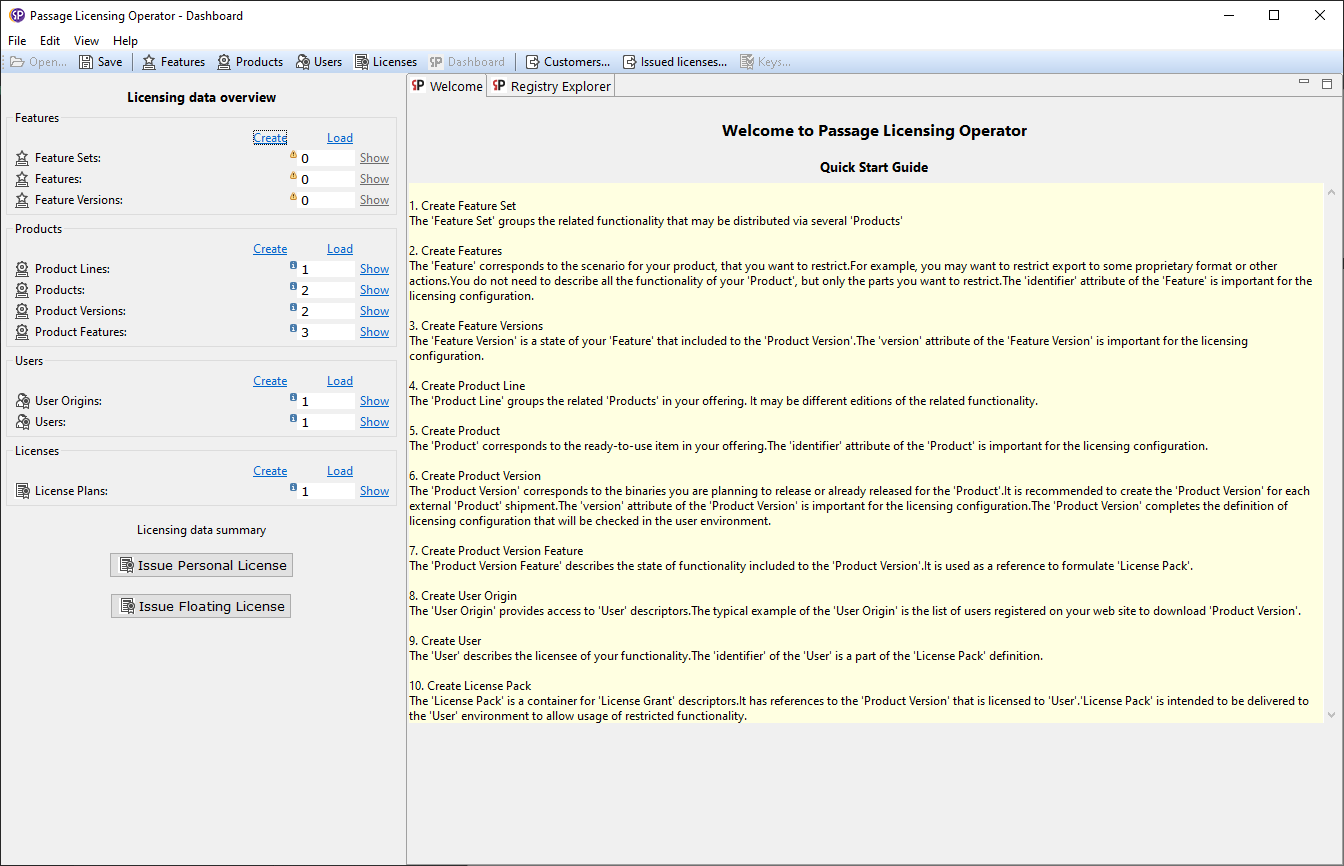
\includegraphics[width=\textwidth]{ui}
\end{center}

\addcontentsline{toc}{section}{How to license your product}
\section*{How to license your product}

This tutorial contains three parts mapped with three licensing steps mentioned in the section above.

\addcontentsline{toc}{subsection}{Definition}
\subsection*{Definition}

First of all, we have to define what our product is. To be more concise with the reader, tutorial at all is provided with examples based on Eclipse Passage commercial version (Cordon).

Usually some products are provided separately around the same system (library or something like that). In our case ArSysOp Cordon provides a simple product line, containing three licensable components:
\begin{itemize}
    \item Cordon Access Cycle (Licensing Components)
    \item Cordon Operator (Like Passage Operator)
    \item Cordon Floating License Server
\end{itemize}

Let's open product line creation dialog by pressing the \textit{Create} button near the Products area.

\begin{center}
    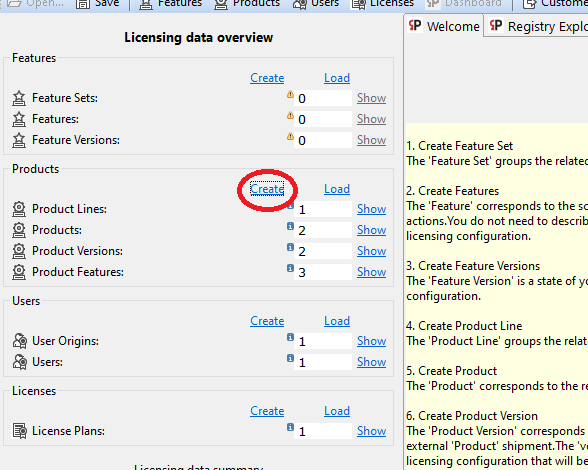
\includegraphics[width=0.75\textwidth]{product_line_create}
\end{center}

In the dialog appeared we have to choose a place, where our product line model will physically exist (as .xmi model), choose unique identifier and any beautiful name.

Remember location where your xmi files are saved. These model files can also be imported with \textit{Load} button.

\begin{center}
    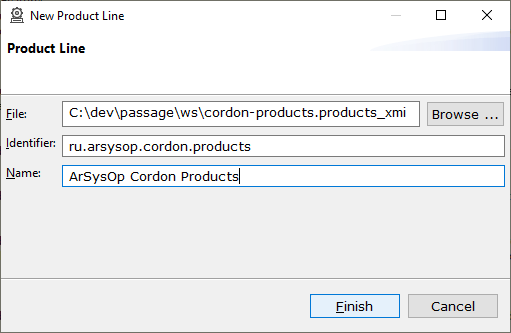
\includegraphics[width=0.75\textwidth]{product_line_dialog}
\end{center}

Press \textit{Finish} and that's it! My congratulations, you have just defined your first product line with Passage! Let's fill it with some products.

Press \textit{Show} near the Product lines count. Now you see the workbench with one defined product line and no products under it.

\begin{center}
    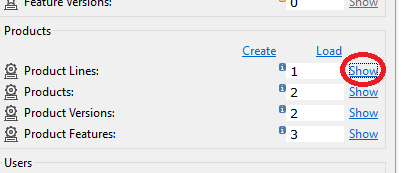
\includegraphics[width=0.75\textwidth]{product_create}
\end{center}

On your product line with right click open the context menu, where you will see an option named \textit{Product}. Pressing it you define new product under the selected product line. 
Let it be the Cordon Operator in our case. Fill all the required fields and optional fields if needed.

\begin{center}
    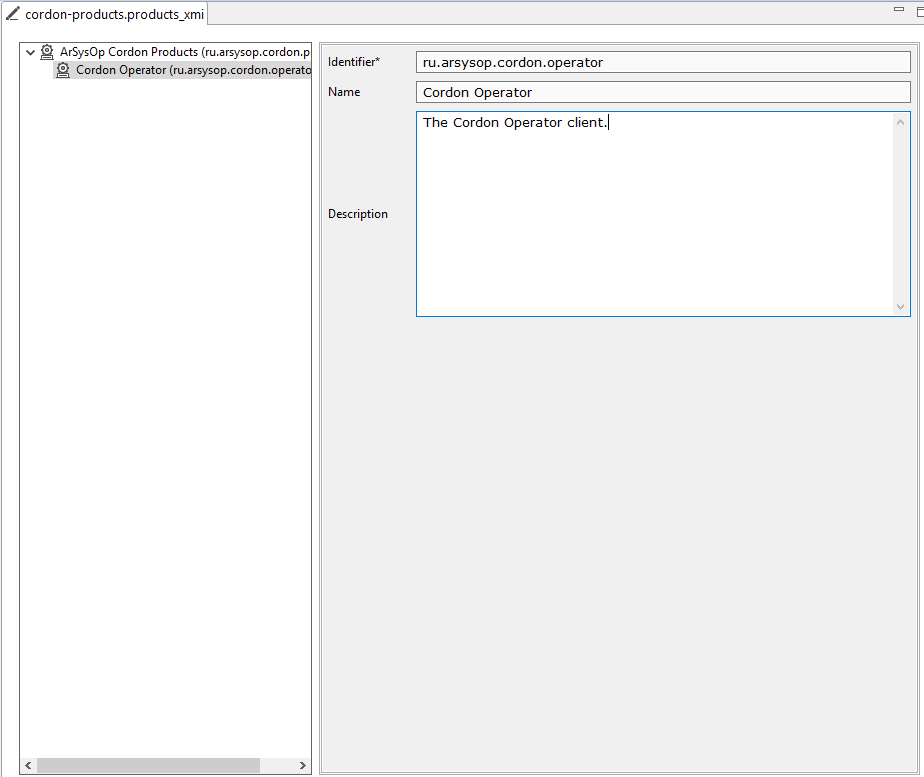
\includegraphics[width=0.75\textwidth]{product_dialog}
\end{center}

Congratulations again! The product is now created and ready to be filled with features, which we are about to define. Let's imagine we have two licensing cases for our product:
\begin{itemize}
    \item we want to check license on start for all users
    \item we want one feature to be licensed separately - not all users who bought Cordon Operator License are allowed to use it. Let it be license usage statistics, for example.
\end{itemize}

First, we have to define a feature that will represent usage statistics collection. Press \textit{Create} button near the Features area to create Feature Set.

\begin{center}
    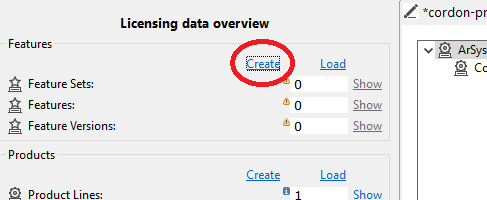
\includegraphics[width=0.75\textwidth]{feature_set_create}
\end{center}

And then select model file location, feature set id and name.

\begin{center}
    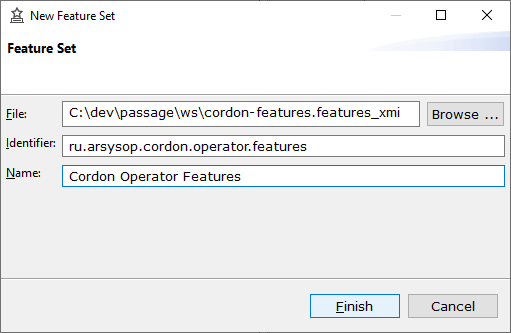
\includegraphics[width=0.75\textwidth]{feature_set_dialog}
\end{center}

Press \textit{Finish} and then \textit{Show} near the feature set count.

\begin{center}
    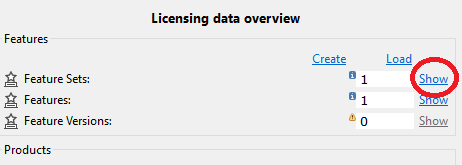
\includegraphics[width=0.75\textwidth]{feature_create}
\end{center}

Like the product under product line, create the feature under feature set with the context menu showed on right-click, then fill identifier and name fields at least and save.

\begin{center}
    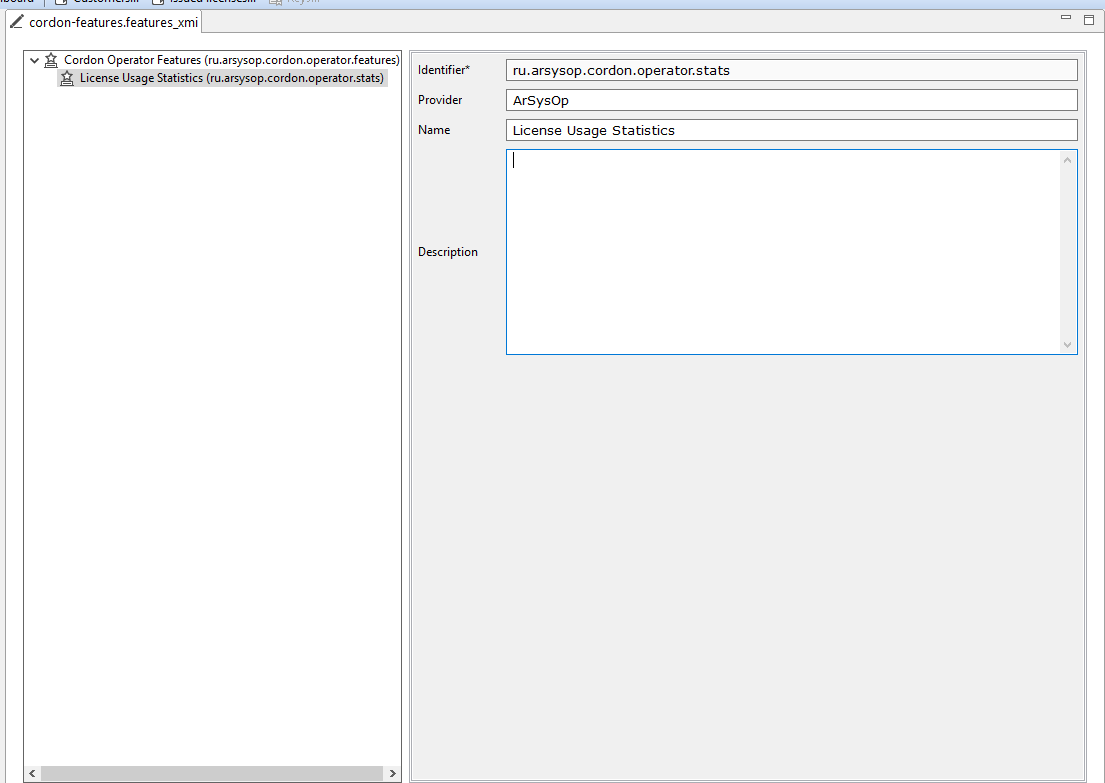
\includegraphics[width=0.75\textwidth]{feature_dialog}
\end{center}

Now we successfully defined our product exceptional feature. To have our product licensed at all, we need to define another feature with \textbf{the same identifier as the product has}. 
Also, developer must use the same identifier when they define their product with Eclipse.

For now we have one product line, one product in it and some exceptional feature to be licensed separately. That's quite enough to proceed to the next part - \textbf{Evolution}.

\addcontentsline{toc}{subsection}{Evolution}
\subsection*{Evolution}



\addcontentsline{toc}{subsection}{Licensing}
\subsection*{Licensing}



\addcontentsline{toc}{chapter}{Glossary}
\chapter*{Glossary}
\markboth{Glossary}{}

\paragraph*{Feature}

\paragraph*{Feature Set}

\paragraph*{Feature Version}

\paragraph*{User}

\paragraph*{User Origin}

\paragraph*{License Plan}

\paragraph*{Product}

\paragraph*{Product Feature}

\paragraph*{Product Line}

\paragraph*{Product Version}

\end{document}